\documentclass[11pt]{article}
\usepackage[paper=letterpaper,margin=1in]{geometry}
\usepackage{mathtools}

\DeclarePairedDelimiter\ceil{\lceil}{\rceil}
\DeclarePairedDelimiter\floor{\lfloor}{\rfloor}
\usepackage[parfill]{parskip}
\usepackage{amsmath}
\usepackage{listings}
\usepackage[obeyspaces,spaces]{url}
\usepackage{graphicx}
\usepackage{tikz}
\usepackage{sourcecodepro}
\usepackage[T1]{fontenc}
\def\CC{{C\nolinebreak[4]\hspace{-.05em}\raisebox{.4ex}{\tiny\bf ++ }}}
\usepackage[
backend=biber,
citestyle=alphabetic,
style=alphabetic,
sorting=ynt
]{biblatex}
\lstset { %
    language=C++,
    backgroundcolor=\color{black!5}, % set backgroundcolor
    basicstyle=\ttfamily\footnotesize,% basic font setting
}
\addbibresource{sample.bib}
\DeclareUrlCommand\class{%
  \renewcommand{\UrlBigBreaks}{\do\.}%
  \renewcommand{\UrlBreaks}{\do\.}%
  }
\DeclareUrlCommand\filedir{%
  \renewcommand{\UrlBigBreaks}{\do\\}%
  \renewcommand{\UrlBreaks}{\do\\}%
  }
\DeclareUrlCommand\method{%
  \renewcommand{\UrlBigBreaks}{}%
  \renewcommand{\UrlBreaks}{}%
  }

\begin{document}
\thispagestyle{empty}
\title{Assignment 406 \\
\large CS 310}
\date{April 2, 2017}
\author{Cameron Moberg}
\maketitle

The heap is a tree-based data structure, where the root is empty or contains a data element of either higher or lower value than both of its children. 
The former is called a \textit{max heap} and the latter a \textit{min heap}.
In this analysis we will exclusively be referring to a \textit{max heap}, and will be analyzing a method that the heap uses: \method{build_heap()}, and a method that is implemented using a heap: \method{heap_sort()}.

For both methods, the value for $n$ is taken to be the number of nodes in the heap.

\section{Build Heap}
To analyze the \method{build_heap()} algorithm, we chose the \method{percolate_down()} method on line 160 as the basic operation because this happens most frequently, is the most expensive, and is the philosophical heart of this algorithm.

However, as it turns out \method{percolate_down()} is the only method called by \method{build_heap()}, and thus we must analyze it in order to find the time complexity of the  \method{build_heap()} method.
\subsection{Percolate Down}

To analyze the \method{percolate_down()} algorithm, we chose both the comparison between child nodes on line 188, and comparison between root and the largest child node on line 195 as the basic operations. This is because they occur most frequently and are the philosophical heart of this algorithm. Regardless of the operation chosen, all of the local work inside of \method{percolate_down()} is linear, will only impact the constants and not the end analysis.

In this algorithm, we assume that the root node's children are heaps, and compare the root node with both of its children. If any of the children are bigger than the root node, we swap values with the largest child, and then recursively call \method{percolate_down()} on the node that we swapped the root with. We repeat this until the root node has no children or is greater than or equal in value to its children.

An empirical analysis of running \method{percolate_down()} for multiple values of $n$ produces the results shown below. Standard function $f(n) = \log n$ with constant multipliers, has been added to illustrate the analysis.

\clearpage
\begin{center}
    % GNUPLOT: LaTeX picture with Postscript
\begingroup
  \makeatletter
  \providecommand\color[2][]{%
    \GenericError{(gnuplot) \space\space\space\@spaces}{%
      Package color not loaded in conjunction with
      terminal option `colourtext'%
    }{See the gnuplot documentation for explanation.%
    }{Either use 'blacktext' in gnuplot or load the package
      color.sty in LaTeX.}%
    \renewcommand\color[2][]{}%
  }%
  \providecommand\includegraphics[2][]{%
    \GenericError{(gnuplot) \space\space\space\@spaces}{%
      Package graphicx or graphics not loaded%
    }{See the gnuplot documentation for explanation.%
    }{The gnuplot epslatex terminal needs graphicx.sty or graphics.sty.}%
    \renewcommand\includegraphics[2][]{}%
  }%
  \providecommand\rotatebox[2]{#2}%
  \@ifundefined{ifGPcolor}{%
    \newif\ifGPcolor
    \GPcolorfalse
  }{}%
  \@ifundefined{ifGPblacktext}{%
    \newif\ifGPblacktext
    \GPblacktexttrue
  }{}%
  % define a \g@addto@macro without @ in the name:
  \let\gplgaddtomacro\g@addto@macro
  % define empty templates for all commands taking text:
  \gdef\gplbacktext{}%
  \gdef\gplfronttext{}%
  \makeatother
  \ifGPblacktext
    % no textcolor at all
    \def\colorrgb#1{}%
    \def\colorgray#1{}%
  \else
    % gray or color?
    \ifGPcolor
      \def\colorrgb#1{\color[rgb]{#1}}%
      \def\colorgray#1{\color[gray]{#1}}%
      \expandafter\def\csname LTw\endcsname{\color{white}}%
      \expandafter\def\csname LTb\endcsname{\color{black}}%
      \expandafter\def\csname LTa\endcsname{\color{black}}%
      \expandafter\def\csname LT0\endcsname{\color[rgb]{1,0,0}}%
      \expandafter\def\csname LT1\endcsname{\color[rgb]{0,1,0}}%
      \expandafter\def\csname LT2\endcsname{\color[rgb]{0,0,1}}%
      \expandafter\def\csname LT3\endcsname{\color[rgb]{1,0,1}}%
      \expandafter\def\csname LT4\endcsname{\color[rgb]{0,1,1}}%
      \expandafter\def\csname LT5\endcsname{\color[rgb]{1,1,0}}%
      \expandafter\def\csname LT6\endcsname{\color[rgb]{0,0,0}}%
      \expandafter\def\csname LT7\endcsname{\color[rgb]{1,0.3,0}}%
      \expandafter\def\csname LT8\endcsname{\color[rgb]{0.5,0.5,0.5}}%
    \else
      % gray
      \def\colorrgb#1{\color{black}}%
      \def\colorgray#1{\color[gray]{#1}}%
      \expandafter\def\csname LTw\endcsname{\color{white}}%
      \expandafter\def\csname LTb\endcsname{\color{black}}%
      \expandafter\def\csname LTa\endcsname{\color{black}}%
      \expandafter\def\csname LT0\endcsname{\color{black}}%
      \expandafter\def\csname LT1\endcsname{\color{black}}%
      \expandafter\def\csname LT2\endcsname{\color{black}}%
      \expandafter\def\csname LT3\endcsname{\color{black}}%
      \expandafter\def\csname LT4\endcsname{\color{black}}%
      \expandafter\def\csname LT5\endcsname{\color{black}}%
      \expandafter\def\csname LT6\endcsname{\color{black}}%
      \expandafter\def\csname LT7\endcsname{\color{black}}%
      \expandafter\def\csname LT8\endcsname{\color{black}}%
    \fi
  \fi
    \setlength{\unitlength}{0.0500bp}%
    \ifx\gptboxheight\undefined%
      \newlength{\gptboxheight}%
      \newlength{\gptboxwidth}%
      \newsavebox{\gptboxtext}%
    \fi%
    \setlength{\fboxrule}{0.5pt}%
    \setlength{\fboxsep}{1pt}%
\begin{picture}(7200.00,5040.00)%
    \gplgaddtomacro\gplbacktext{%
      \csname LTb\endcsname%
      \put(682,704){\makebox(0,0)[r]{\strut{}$0$}}%
      \put(682,1623){\makebox(0,0)[r]{\strut{}$5$}}%
      \put(682,2542){\makebox(0,0)[r]{\strut{}$10$}}%
      \put(682,3460){\makebox(0,0)[r]{\strut{}$15$}}%
      \put(682,4379){\makebox(0,0)[r]{\strut{}$20$}}%
      \put(1402,484){\makebox(0,0){\strut{}$500$}}%
      \put(2002,484){\makebox(0,0){\strut{}$1000$}}%
      \put(2602,484){\makebox(0,0){\strut{}$1500$}}%
      \put(3202,484){\makebox(0,0){\strut{}$2000$}}%
      \put(3802,484){\makebox(0,0){\strut{}$2500$}}%
      \put(4403,484){\makebox(0,0){\strut{}$3000$}}%
      \put(5003,484){\makebox(0,0){\strut{}$3500$}}%
      \put(5603,484){\makebox(0,0){\strut{}$4000$}}%
      \put(6203,484){\makebox(0,0){\strut{}$4500$}}%
      \put(6803,484){\makebox(0,0){\strut{}$5000$}}%
      \put(3202,3800){\rotatebox{7}{\makebox(0,0)[l]{\strut{}$\frac{3}{2} \log(n)$}}}%
    }%
    \gplgaddtomacro\gplfronttext{%
      \csname LTb\endcsname%
      \put(176,2541){\rotatebox{-270}{\makebox(0,0){\strut{}Operation Count}}}%
      \put(3808,154){\makebox(0,0){\strut{}Input Size}}%
      \put(3808,4709){\makebox(0,0){\strut{}Empirical Analysis of Percolate Down Algorithm}}%
    }%
    \gplbacktext
    \put(0,0){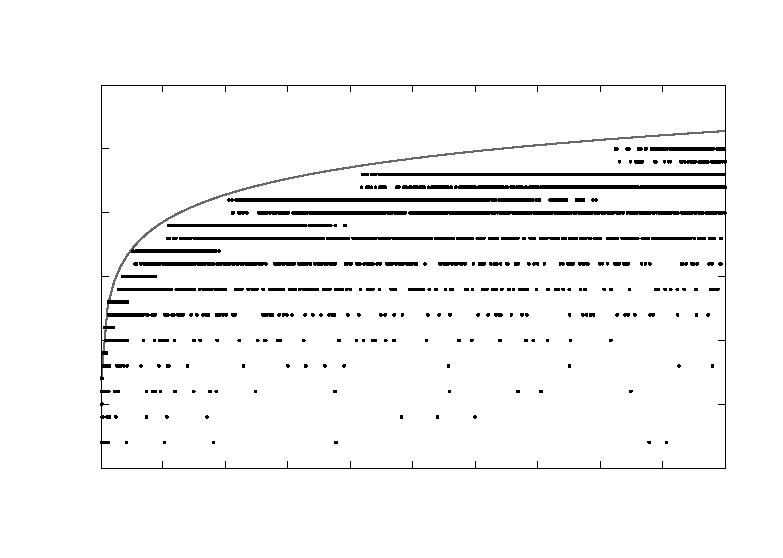
\includegraphics{perc}}%
    \gplfronttext
  \end{picture}%
\endgroup

\end{center}

The \CC method used to produce this:

\begin{lstlisting}
    void empiric_perc( Comparable key )
    {
        heap.at( 0 ) = key; 	  //heap is a max_heap by definition.
        heap.percolate_down( 0 ); //0 is the root node index.
    }
\end{lstlisting}

In short, we set $key$ to a generated (pseudo) random number, then we set the root node of the heap equal to it, and then \method{percolate_down()} was called with the root node index in order to simulate a ``worst case scenario".

An examination of the \method{percolate_down()} method itself explains the empirical results when we observe that if the root node's value is the smallest of all nodes in the tree, it will have to end up as a leaf, at the bottom of the tree. This requires a comparison at every level of the tree, or, $\log n$ comparisons.

Since this algorithm can end early, we cannot tighten the bound to Big-$\Theta$, and thus the \method{percolate_down()} algorithm can be described as 

\[
T(n) \in O( \log n)
\]
\[
T(n) \in \Omega(1)
\]
\clearpage
\subsection{Build Heap cont.}

An empirical analysis of running \method{build_heap()} with multiple values of $n$ produces the results shown below. Standard function $f(n) = n$ with constant multipliers, has been added to

\begin{center}
    % GNUPLOT: LaTeX picture with Postscript
\begingroup
  \makeatletter
  \providecommand\color[2][]{%
    \GenericError{(gnuplot) \space\space\space\@spaces}{%
      Package color not loaded in conjunction with
      terminal option `colourtext'%
    }{See the gnuplot documentation for explanation.%
    }{Either use 'blacktext' in gnuplot or load the package
      color.sty in LaTeX.}%
    \renewcommand\color[2][]{}%
  }%
  \providecommand\includegraphics[2][]{%
    \GenericError{(gnuplot) \space\space\space\@spaces}{%
      Package graphicx or graphics not loaded%
    }{See the gnuplot documentation for explanation.%
    }{The gnuplot epslatex terminal needs graphicx.sty or graphics.sty.}%
    \renewcommand\includegraphics[2][]{}%
  }%
  \providecommand\rotatebox[2]{#2}%
  \@ifundefined{ifGPcolor}{%
    \newif\ifGPcolor
    \GPcolorfalse
  }{}%
  \@ifundefined{ifGPblacktext}{%
    \newif\ifGPblacktext
    \GPblacktexttrue
  }{}%
  % define a \g@addto@macro without @ in the name:
  \let\gplgaddtomacro\g@addto@macro
  % define empty templates for all commands taking text:
  \gdef\gplbacktext{}%
  \gdef\gplfronttext{}%
  \makeatother
  \ifGPblacktext
    % no textcolor at all
    \def\colorrgb#1{}%
    \def\colorgray#1{}%
  \else
    % gray or color?
    \ifGPcolor
      \def\colorrgb#1{\color[rgb]{#1}}%
      \def\colorgray#1{\color[gray]{#1}}%
      \expandafter\def\csname LTw\endcsname{\color{white}}%
      \expandafter\def\csname LTb\endcsname{\color{black}}%
      \expandafter\def\csname LTa\endcsname{\color{black}}%
      \expandafter\def\csname LT0\endcsname{\color[rgb]{1,0,0}}%
      \expandafter\def\csname LT1\endcsname{\color[rgb]{0,1,0}}%
      \expandafter\def\csname LT2\endcsname{\color[rgb]{0,0,1}}%
      \expandafter\def\csname LT3\endcsname{\color[rgb]{1,0,1}}%
      \expandafter\def\csname LT4\endcsname{\color[rgb]{0,1,1}}%
      \expandafter\def\csname LT5\endcsname{\color[rgb]{1,1,0}}%
      \expandafter\def\csname LT6\endcsname{\color[rgb]{0,0,0}}%
      \expandafter\def\csname LT7\endcsname{\color[rgb]{1,0.3,0}}%
      \expandafter\def\csname LT8\endcsname{\color[rgb]{0.5,0.5,0.5}}%
    \else
      % gray
      \def\colorrgb#1{\color{black}}%
      \def\colorgray#1{\color[gray]{#1}}%
      \expandafter\def\csname LTw\endcsname{\color{white}}%
      \expandafter\def\csname LTb\endcsname{\color{black}}%
      \expandafter\def\csname LTa\endcsname{\color{black}}%
      \expandafter\def\csname LT0\endcsname{\color{black}}%
      \expandafter\def\csname LT1\endcsname{\color{black}}%
      \expandafter\def\csname LT2\endcsname{\color{black}}%
      \expandafter\def\csname LT3\endcsname{\color{black}}%
      \expandafter\def\csname LT4\endcsname{\color{black}}%
      \expandafter\def\csname LT5\endcsname{\color{black}}%
      \expandafter\def\csname LT6\endcsname{\color{black}}%
      \expandafter\def\csname LT7\endcsname{\color{black}}%
      \expandafter\def\csname LT8\endcsname{\color{black}}%
    \fi
  \fi
    \setlength{\unitlength}{0.0500bp}%
    \ifx\gptboxheight\undefined%
      \newlength{\gptboxheight}%
      \newlength{\gptboxwidth}%
      \newsavebox{\gptboxtext}%
    \fi%
    \setlength{\fboxrule}{0.5pt}%
    \setlength{\fboxsep}{1pt}%
\begin{picture}(7200.00,5040.00)%
    \gplgaddtomacro\gplbacktext{%
      \csname LTb\endcsname%
      \put(1078,704){\makebox(0,0)[r]{\strut{}$0$}}%
      \put(1078,1072){\makebox(0,0)[r]{\strut{}$1000$}}%
      \put(1078,1439){\makebox(0,0)[r]{\strut{}$2000$}}%
      \put(1078,1807){\makebox(0,0)[r]{\strut{}$3000$}}%
      \put(1078,2174){\makebox(0,0)[r]{\strut{}$4000$}}%
      \put(1078,2542){\makebox(0,0)[r]{\strut{}$5000$}}%
      \put(1078,2909){\makebox(0,0)[r]{\strut{}$6000$}}%
      \put(1078,3277){\makebox(0,0)[r]{\strut{}$7000$}}%
      \put(1078,3644){\makebox(0,0)[r]{\strut{}$8000$}}%
      \put(1078,4012){\makebox(0,0)[r]{\strut{}$9000$}}%
      \put(1078,4379){\makebox(0,0)[r]{\strut{}$10000$}}%
      \put(1210,484){\makebox(0,0){\strut{}$0$}}%
      \put(1769,484){\makebox(0,0){\strut{}$500$}}%
      \put(2329,484){\makebox(0,0){\strut{}$1000$}}%
      \put(2888,484){\makebox(0,0){\strut{}$1500$}}%
      \put(3447,484){\makebox(0,0){\strut{}$2000$}}%
      \put(4007,484){\makebox(0,0){\strut{}$2500$}}%
      \put(4566,484){\makebox(0,0){\strut{}$3000$}}%
      \put(5125,484){\makebox(0,0){\strut{}$3500$}}%
      \put(5684,484){\makebox(0,0){\strut{}$4000$}}%
      \put(6244,484){\makebox(0,0){\strut{}$4500$}}%
      \put(6803,484){\makebox(0,0){\strut{}$5000$}}%
      \put(2888,1929){\rotatebox{37}{\makebox(0,0)[l]{\strut{}$2n$}}}%
      \put(3447,1750){\rotatebox{33}{\makebox(0,0)[l]{\strut{}$\frac{7}{8} n$}}}%
    }%
    \gplgaddtomacro\gplfronttext{%
      \csname LTb\endcsname%
      \put(176,2541){\rotatebox{-270}{\makebox(0,0){\strut{}Operation Count}}}%
      \put(4006,154){\makebox(0,0){\strut{}Input Size}}%
      \put(4006,4709){\makebox(0,0){\strut{}\textbf{Empirical Analysis of Build Heap Algorithm}}}%
    }%
    \gplbacktext
    \put(0,0){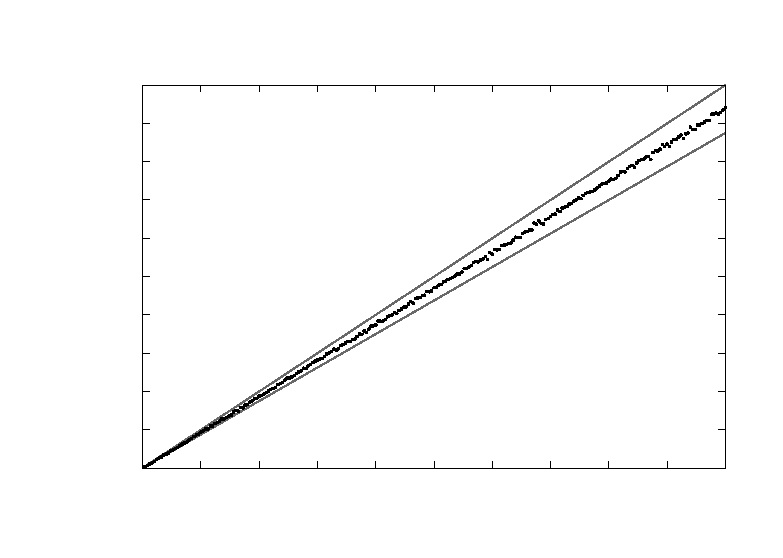
\includegraphics{build}}%
    \gplfronttext
  \end{picture}%
\endgroup

\end{center}

At first glance, it would appear that the algorithm is described by $O(n \log n)$ since there is a single deterministic loop that iterates $\frac{n}{2} - 1$ times containing a $O(\log n)$ method. This is technically correct, but not the best we can do.
Upon closer inspection we can tighten the bound to $O(n)$.

This is because of the fact that most of the work is comparisons are done on the lower levels, where there are less total comparisons than the higher levels. In a full binary tree there are $n=2^{h+1}-1$ nodes, where $h$ is the height of the tree. The number of comparisons in \method{build_heap()} is shown below.
\begin{center}
 \begin{tabular}{||c c c||} 
 \hline
 Depth of Nodes &  Height of Nodes & Num. of Comparisons \\ [0.5ex] 
 \hline
 \hline
 $h$ & 0 & 0 \\
 \hline 
 
 $h-1$ & 1 & $2 \frac{n}{4}$  \\ 
 \hline
 
 $h-2$ & 2 & $2(\frac{n}{8} + \frac{n}{4})$  \\
 \hline
 
 $h-3$ & 3 & $2(\frac{n}{16} + \frac{n}{8} + \frac{n}{4})$   \\
 \hline
 
 ... & ... & ...  \\
 \hline
\end{tabular}
\end{center}

When \method{build_heap()} runs on a full binary tree, it starts on the level one above all of the leaves, as the leaves will have 0 comparisons, and iterates through calling \method{percolate_down()} on every node in reverse level order. The worst case amount of operations done is equivalent to the summation shown below.
\[
	\sum_{i=1}^{h}\frac{2(n+1)}{2^{i+1}} \in O(n)
\]


The summation, although not done in this analysis, can be shown to be linear. Also, realize that the algorithm must access every element of the array at least once, which gives it $\Omega(n)$ time. Therefore, we conclude that the algorithm is of the form
\[
	T(n)\in \Theta(n)
\]
The author never explicitly stated what efficiency class the algorithm is in, but it can be assumed that they concluded that it is $O(n)$ \cite[230]{levit}. Our analysis does agree with the author's up to a point, but by observing that the algorithm must be $\Omega(n)$ we can tighten the bound to Big-$\Theta$, instead of just Big-$O$.

\section{Heap Sort}

In general, a heap sort algorithm contains two major parts: building a heap from data, and repeatedly removing the root node and inserting it into the to-be-sorted array. As shown above, the first part can be done in linear time.

To analyze the \method{heap_sort()} algorithm, we chose \method{delete_max()} method on line 118 as the basic operation because this occurs most frequently and is the philosophical heart of this algorithm. We also chose this method because it has already been shown in this analysis that the first part of the sort, building the heap, is $\Theta(n)$ time, and only happens once.

An empirical analysis of running \method{heap_sort()} for multiple values of $n$ produces the results shown below. Standard function $f(n) = n \log n$ with constant multipliers, has been added to illustrate the analysis.

\begin{center}
    % GNUPLOT: LaTeX picture with Postscript
\begingroup
  \makeatletter
  \providecommand\color[2][]{%
    \GenericError{(gnuplot) \space\space\space\@spaces}{%
      Package color not loaded in conjunction with
      terminal option `colourtext'%
    }{See the gnuplot documentation for explanation.%
    }{Either use 'blacktext' in gnuplot or load the package
      color.sty in LaTeX.}%
    \renewcommand\color[2][]{}%
  }%
  \providecommand\includegraphics[2][]{%
    \GenericError{(gnuplot) \space\space\space\@spaces}{%
      Package graphicx or graphics not loaded%
    }{See the gnuplot documentation for explanation.%
    }{The gnuplot epslatex terminal needs graphicx.sty or graphics.sty.}%
    \renewcommand\includegraphics[2][]{}%
  }%
  \providecommand\rotatebox[2]{#2}%
  \@ifundefined{ifGPcolor}{%
    \newif\ifGPcolor
    \GPcolorfalse
  }{}%
  \@ifundefined{ifGPblacktext}{%
    \newif\ifGPblacktext
    \GPblacktexttrue
  }{}%
  % define a \g@addto@macro without @ in the name:
  \let\gplgaddtomacro\g@addto@macro
  % define empty templates for all commands taking text:
  \gdef\gplbacktext{}%
  \gdef\gplfronttext{}%
  \makeatother
  \ifGPblacktext
    % no textcolor at all
    \def\colorrgb#1{}%
    \def\colorgray#1{}%
  \else
    % gray or color?
    \ifGPcolor
      \def\colorrgb#1{\color[rgb]{#1}}%
      \def\colorgray#1{\color[gray]{#1}}%
      \expandafter\def\csname LTw\endcsname{\color{white}}%
      \expandafter\def\csname LTb\endcsname{\color{black}}%
      \expandafter\def\csname LTa\endcsname{\color{black}}%
      \expandafter\def\csname LT0\endcsname{\color[rgb]{1,0,0}}%
      \expandafter\def\csname LT1\endcsname{\color[rgb]{0,1,0}}%
      \expandafter\def\csname LT2\endcsname{\color[rgb]{0,0,1}}%
      \expandafter\def\csname LT3\endcsname{\color[rgb]{1,0,1}}%
      \expandafter\def\csname LT4\endcsname{\color[rgb]{0,1,1}}%
      \expandafter\def\csname LT5\endcsname{\color[rgb]{1,1,0}}%
      \expandafter\def\csname LT6\endcsname{\color[rgb]{0,0,0}}%
      \expandafter\def\csname LT7\endcsname{\color[rgb]{1,0.3,0}}%
      \expandafter\def\csname LT8\endcsname{\color[rgb]{0.5,0.5,0.5}}%
    \else
      % gray
      \def\colorrgb#1{\color{black}}%
      \def\colorgray#1{\color[gray]{#1}}%
      \expandafter\def\csname LTw\endcsname{\color{white}}%
      \expandafter\def\csname LTb\endcsname{\color{black}}%
      \expandafter\def\csname LTa\endcsname{\color{black}}%
      \expandafter\def\csname LT0\endcsname{\color{black}}%
      \expandafter\def\csname LT1\endcsname{\color{black}}%
      \expandafter\def\csname LT2\endcsname{\color{black}}%
      \expandafter\def\csname LT3\endcsname{\color{black}}%
      \expandafter\def\csname LT4\endcsname{\color{black}}%
      \expandafter\def\csname LT5\endcsname{\color{black}}%
      \expandafter\def\csname LT6\endcsname{\color{black}}%
      \expandafter\def\csname LT7\endcsname{\color{black}}%
      \expandafter\def\csname LT8\endcsname{\color{black}}%
    \fi
  \fi
    \setlength{\unitlength}{0.0500bp}%
    \ifx\gptboxheight\undefined%
      \newlength{\gptboxheight}%
      \newlength{\gptboxwidth}%
      \newsavebox{\gptboxtext}%
    \fi%
    \setlength{\fboxrule}{0.5pt}%
    \setlength{\fboxsep}{1pt}%
\begin{picture}(7200.00,5040.00)%
    \gplgaddtomacro\gplbacktext{%
      \csname LTb\endcsname%
      \put(1210,704){\makebox(0,0)[r]{\strut{}$0$}}%
      \put(1210,1317){\makebox(0,0)[r]{\strut{}$20000$}}%
      \put(1210,1929){\makebox(0,0)[r]{\strut{}$40000$}}%
      \put(1210,2542){\makebox(0,0)[r]{\strut{}$60000$}}%
      \put(1210,3154){\makebox(0,0)[r]{\strut{}$80000$}}%
      \put(1210,3767){\makebox(0,0)[r]{\strut{}$100000$}}%
      \put(1210,4379){\makebox(0,0)[r]{\strut{}$120000$}}%
      \put(1342,484){\makebox(0,0){\strut{}$0$}}%
      \put(1888,484){\makebox(0,0){\strut{}$500$}}%
      \put(2434,484){\makebox(0,0){\strut{}$1000$}}%
      \put(2980,484){\makebox(0,0){\strut{}$1500$}}%
      \put(3526,484){\makebox(0,0){\strut{}$2000$}}%
      \put(4073,484){\makebox(0,0){\strut{}$2500$}}%
      \put(4619,484){\makebox(0,0){\strut{}$3000$}}%
      \put(5165,484){\makebox(0,0){\strut{}$3500$}}%
      \put(5711,484){\makebox(0,0){\strut{}$4000$}}%
      \put(6257,484){\makebox(0,0){\strut{}$4500$}}%
      \put(6803,484){\makebox(0,0){\strut{}$5000$}}%
      \put(2980,1720){\rotatebox{31}{\makebox(0,0)[l]{\strut{}$\frac{5}{2} n\log n$}}}%
      \put(3526,1480){\rotatebox{27}{\makebox(0,0)[l]{\strut{}$2n \log n$}}}%
    }%
    \gplgaddtomacro\gplfronttext{%
      \csname LTb\endcsname%
      \put(176,2541){\rotatebox{-270}{\makebox(0,0){\strut{}Operation Count}}}%
      \put(4072,154){\makebox(0,0){\strut{}Input Size}}%
      \put(4072,4709){\makebox(0,0){\strut{}\textbf{Empirical Analysis of Heap Sort Algorithm}}}%
    }%
    \gplbacktext
    \put(0,0){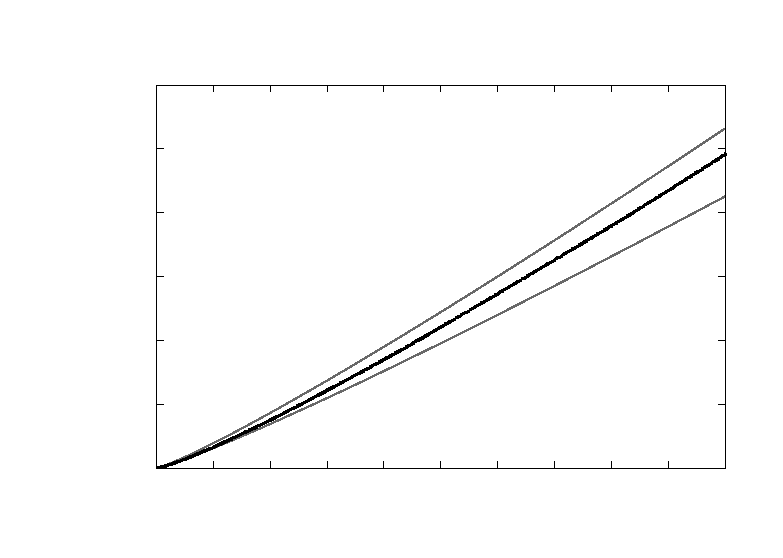
\includegraphics{sort}}%
    \gplfronttext
  \end{picture}%
\endgroup

\end{center}

An examination of the code itself explains the empirical results when we observe that this algorithm is calls the method \method{delete_max()}, which in turn has constant work, except for the call to \method{percolate_down()}, which has been shown above to be $O(\log n)$ time. If we go back and take a look at \method{heap_sort()}, there is a deterministic for loop that runs approximately $n/2$ times. When we combine these two facts, we get that \method{heap_sort()} is of the form
\[
	T(n)\in O(n\log n)
\]
	
We cannot tighten the bound to Big-$\Theta$ because of the fact that \method{percolate_down()} is not Big-$\Theta$.
\nocite{*}
\clearpage
\printbibliography
\end{document}